\documentclass{standalone}
\usepackage{tikz}
\usetikzlibrary{positioning, arrows, shapes.gates.logic.US, calc}

% This is just an and gate from the shapes.gates.logic.US library
% Note I'm using 3 inputs
\tikzset{
        my-and-gate/.style={
            and gate US, draw, rotate=0, logic gate inputs=nnn, very thick
        },
}

\begin{document}

\resizebox{10cm}{6cm}{

    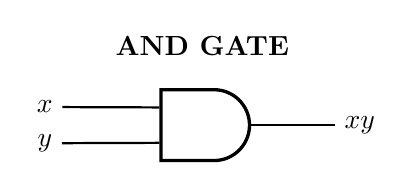
\begin{tikzpicture}[node distance=.2cm]

        %DRAW NODES (I like to do them relative to each other, In this case the AND gate)
        \node [my-and-gate]   (AND)  at (0,0)                  {};
        \node []              (X)    at ($(AND)+(-2.0,.23)$)   {\normalsize $x$};
        \node []              (Y)    at ($(AND)+(-2.0,-.23)$)  {\normalsize $y$};
        \node []              (XY)   at ($(AND)+(2.0,0)$)      {\normalsize $xy$};
        \node []              (NAME) at ($(AND)+(0,1.0)$)      {\normalsize \textbf {AND GATE}};

        % CONNECT INPUTS
        \draw [thick] (X) -- (AND.input 1);
        \draw [thick] (Y) -- (AND.input 3);

        % CONNECT OUTPUTS
        \draw [thick] (AND.output) -- (XY);

    \end{tikzpicture}
}

\end{document} 
